\section{Node specifikationer}

\begin{figure}[H]
	\centering
	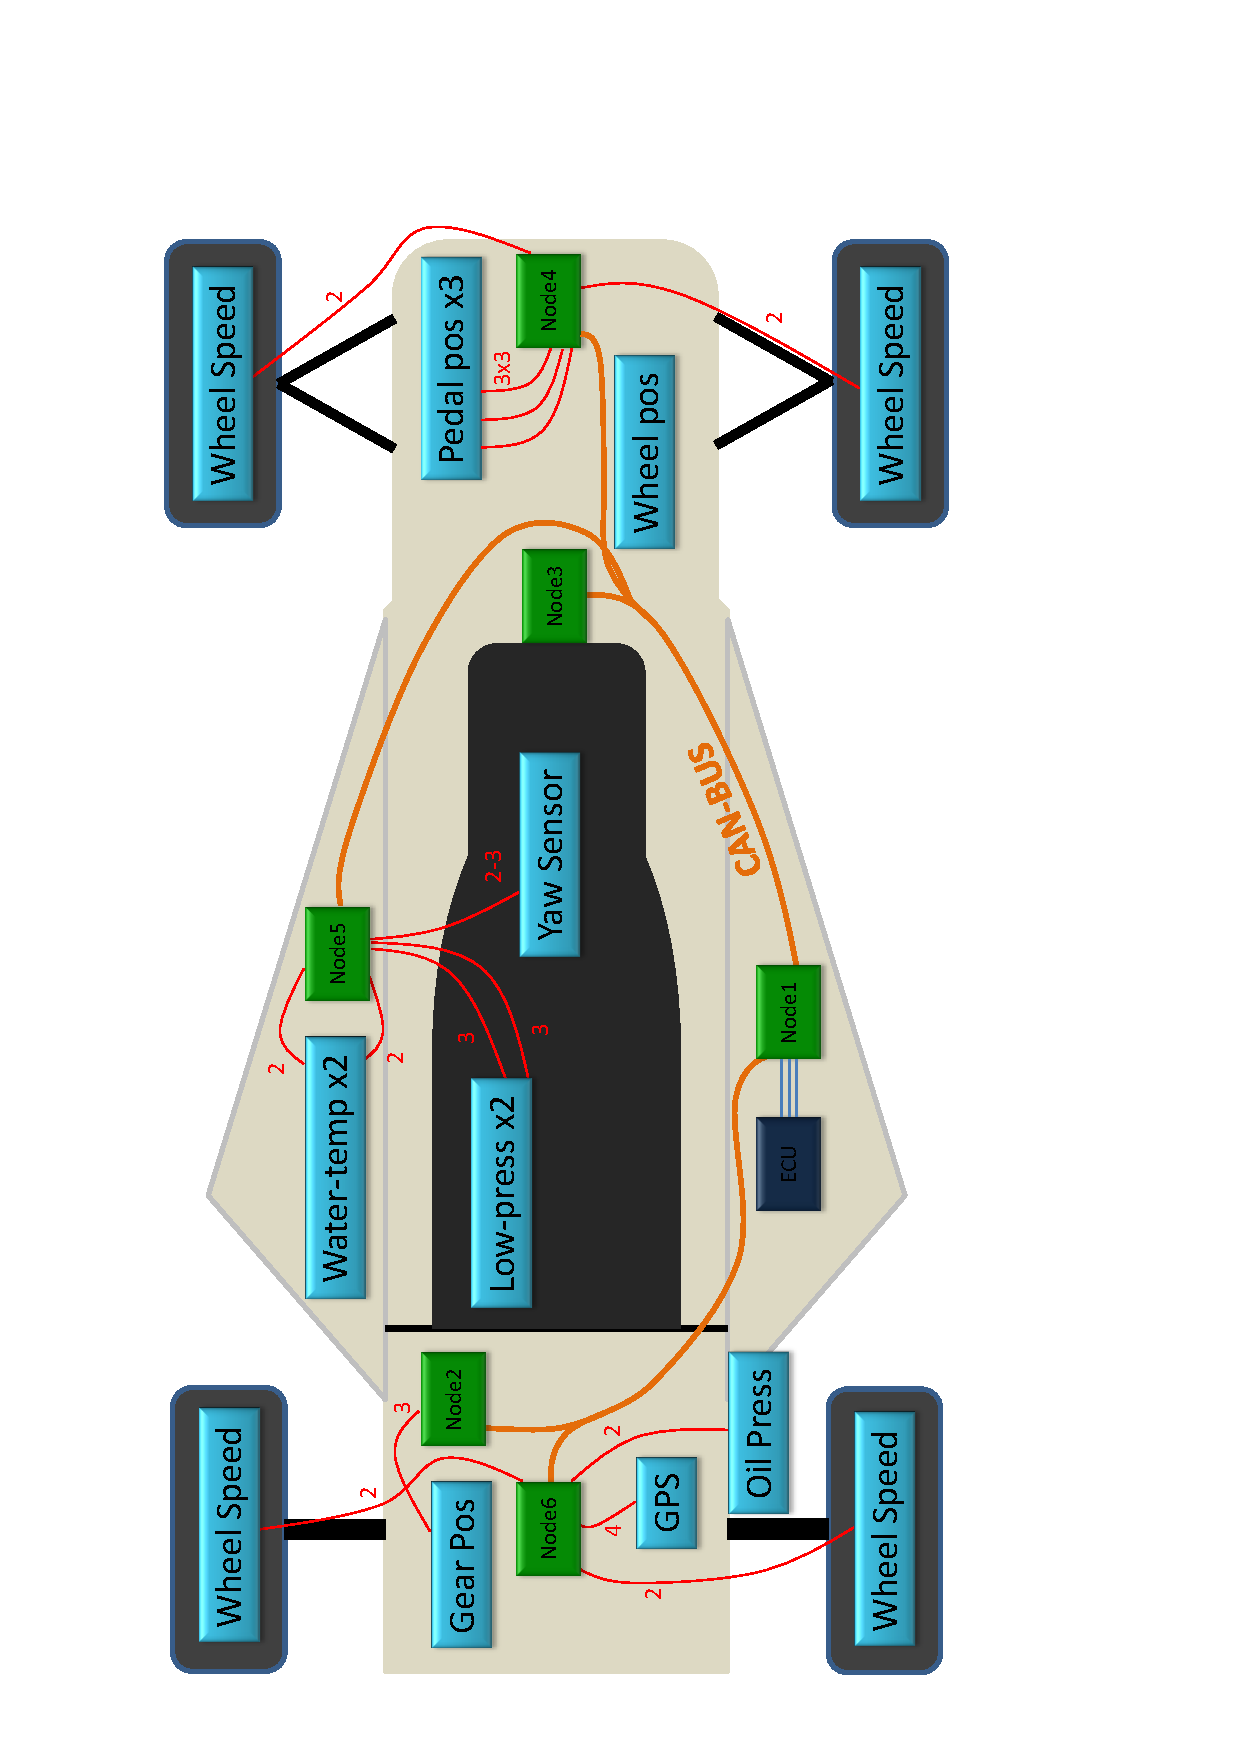
\includegraphics[width=0.8\textwidth, angle=270]{../software/noder/diagram_car.pdf}
	\caption{Diagram over noder på bil.\label{fig:bil_diagram}}
\end{figure}

\begin{table}[H] \centering
	\begin{tabular}{|c|c|c|c|c|}
        \hline \multicolumn{5}{|c|}{\textbf{Node 4}} \\
	    \hline \hline \textbf{Sensor} & \textbf{Antal} & \textbf{Data size [bit]} & \textbf{Total [bit]} & \textbf{Updateringsrate [Hz]}\\
        \hline Speeder pedal pos & 1 & 8 & 8 & 20 ? \\
        \hline Break pedal pos & 1 & 8 & 8 & 20 ? \\
        \hline Clutch pedal pos & 1 & 8 & 8 & 20 ? \\
        \hline Steering wheel pos & 1 & 8 & 8 & 20 ? \\
        \hline Wheel speed front & 2 & 8 & 16 & 50 ? \\
        \hline
    \end{tabular}
\caption{Node 4 sensor specifikation.}
\label{table:CAN_node4}
\end{table}

\begin{table}[H] \centering
	\begin{tabular}{|c|c|c|c|c|}
        \hline \multicolumn{5}{|c|}{\textbf{Node 5}} \\
	    \hline \hline \textbf{Sensor} & \textbf{Antal} & \textbf{Data size [bit]} & \textbf{Total [bit]} & \textbf{Updateringsrate [Hz]}\\
        \hline Low-press & 2 &  8 & 16 & 10 ? \\
        \hline Yaw & 1 & 30 & 30 & 30 ? \\
        \hline Water-temp & 2 &  8 & 16 & 1 \\
        \hline
    \end{tabular}
\caption{Node 5 sensor specifikation.}
\label{table:CAN_node5}
\end{table}

\begin{table}[H] \centering
	\begin{tabular}{|c|c|c|c|c|}
        \hline \multicolumn{5}{|c|}{\textbf{Node 6}} \\
	    \hline \hline \textbf{Sensor} & \textbf{Antal} & \textbf{Data size [bit]} & \textbf{Total [bit]} & \textbf{Updateringsrate [Hz]}\\
        \hline Wheel speed back & 2 &  8 & 16 & 50 ?\\
        \hline Olie press & 1 &  8 & 8 & 10\\
        \hline GPS & 1 &  40 ? & 40 ? & < 5 ?\\
        \hline
    \end{tabular}
\caption{Node 6 sensor specifikation.}
\label{table:CAN_node6}
\end{table}
